\chapter{Introduction}
\section{Overview}
\subsection{Wireless Sensor Network Overview}
Recent advances in micro-electro-mechanical systems, embedded processors, and wireless communications have led to the emergence of Wireless sensor networks (WSNs) \cite{wsn-survey}, which consist of a large number of sensing devices each capable of sensing, processing and transmitting environmental information. Applications of wireless sensor network include battlefield surveillance \cite{wsn-app}, biological detection, smart spaces \cite{wsn-app}, industrial diagnostics, and so on. Another important application of wireless sensor network that cannot be left out is environmental monitoring, analyzing and forecasting disasters such as Forest fire detection, Flood detection, ... We envision that, in near future, wireless sensor networks will be more popular and be an integral part of our lives.

One of the most important constraints on sensor nodes is the low power consumption requirement. The wireless sensor node can only be equipped with a limited, generally irreplaceable, power source. Therefore, while traditional networks aim to achieve high quality of service (QoS), sensor network protocols must focus primarily on power conservation. In an ad hoc sensor network, each node plays the dual role of data originator and data router. The dis-functioning of few nodes can cause significant topological changes and might require re-routing of packets. Hence, power conservation and power management take on additional importance.

Another essential property of wireless sensor networks is its scalability and distribution. The number of sensor nodes deployed in studying a phenomenon may be in the order of hundreds or thousands. Depending on the application, the number may reach an extreme value of millions, for instance, the forest fire detection system may contain thousands sensor nodes.

In the wireless sensor network, communicating nodes are linked by a wireless medium. Thus, a sensor node can only communicate with sensor nodes which lie within its communication range. In case of communicating two sensor nodes which do not lie within each other's communication range, the packet have to be transmitted via intermediate nodes. The routing path of packets is calculated depending on the routing protocol that network uses.


\subsection{Geographical routing in Wireless Sensor Network}
Routing protocols in wireless sensor network recently has attracted much concerns from researchers. The designing of routing protocols in wireless sensor network is challenging due to its mentioned properties. For example, in the traditional network such as Ethernet, a node can analysis whole network to find out the optimal routing path, however, it is impossible to do this task in wireless sensor network. The requirements of routing protocols in wireless sensor network not only includes low latency, fault tolerance, but also has to guarantee following factors:

\begin{itemize}
\item \emph{Computational complexity}: sensor nodes have very limited and low hardware power so the complexity of the algorithm has to be as simple as possible. For example, the wide use sensor node, Mica 2 Mote \cite{mica2}, has only 128K bytes of program flash memory and uses a 8-bit micro-controller.
\item \emph{Energy consumption}: because of limited and irreplaceable power source, the routing protocol has to be energy efficiency.
\item \emph{Load balancing}: the load balance has a big impact on the energy consumption of sensor nodes. Network congestion causes some sensor nodes carry more data than the others and quickly die. Consequently, it significantly changes the connectivity and topology of the network. Thus, load balancing plays an important role in routing in wireless sensor networks.
\end{itemize} 

A common approach is using geographical location information of sensor nodes to design the routing protocols. It is well suited for large-scale wireless sensor networks because it is nearly stateless. The class of these protocols is named \emph{geographical routing protocols}. This approach assumes that exact location of sensor nodes is known beforehand. In other words, the routing path of the packet is conducted from the geographical location information of sensor nodes. Notice that, in geographical routing, each sensor node only needs to know its neighbors' location information (a 1-hop neighbor of a sensor node \emph{S} is a node which is inside the communication range of \emph{S}). When a sensor node receives a packet, it decides to forward this packet to one of its neighbors based on current location information of its neighbors. 

A classical algorithm in this type of protocols is the greedy algorithm \cite{wsn-greedy}. The greedy algorithm is described as follows: the packet is forwarded to a neighbor which is closer to the destination node than current node and closest to the destination node among all neighbor nodes. Greedy forwarding’s great advantage is its reliance only on knowledge of the forwarding node’s immediate neighbors. The state required is negligible, and dependent on the density of nodes in the wireless network, not the total number of destinations in the network. However, the biggest problem of greedy algorithm is the occurrence of the local minimum phenomenon, i.e. there is no satisfying neighbor to forward the packet anymore. Figure \ref{local-minimum} demonstrates this phenomenon. This problems is usually caused by the existence of \emph{routing holes} in the network topology.
\begin{figure}[!htb]
\centering
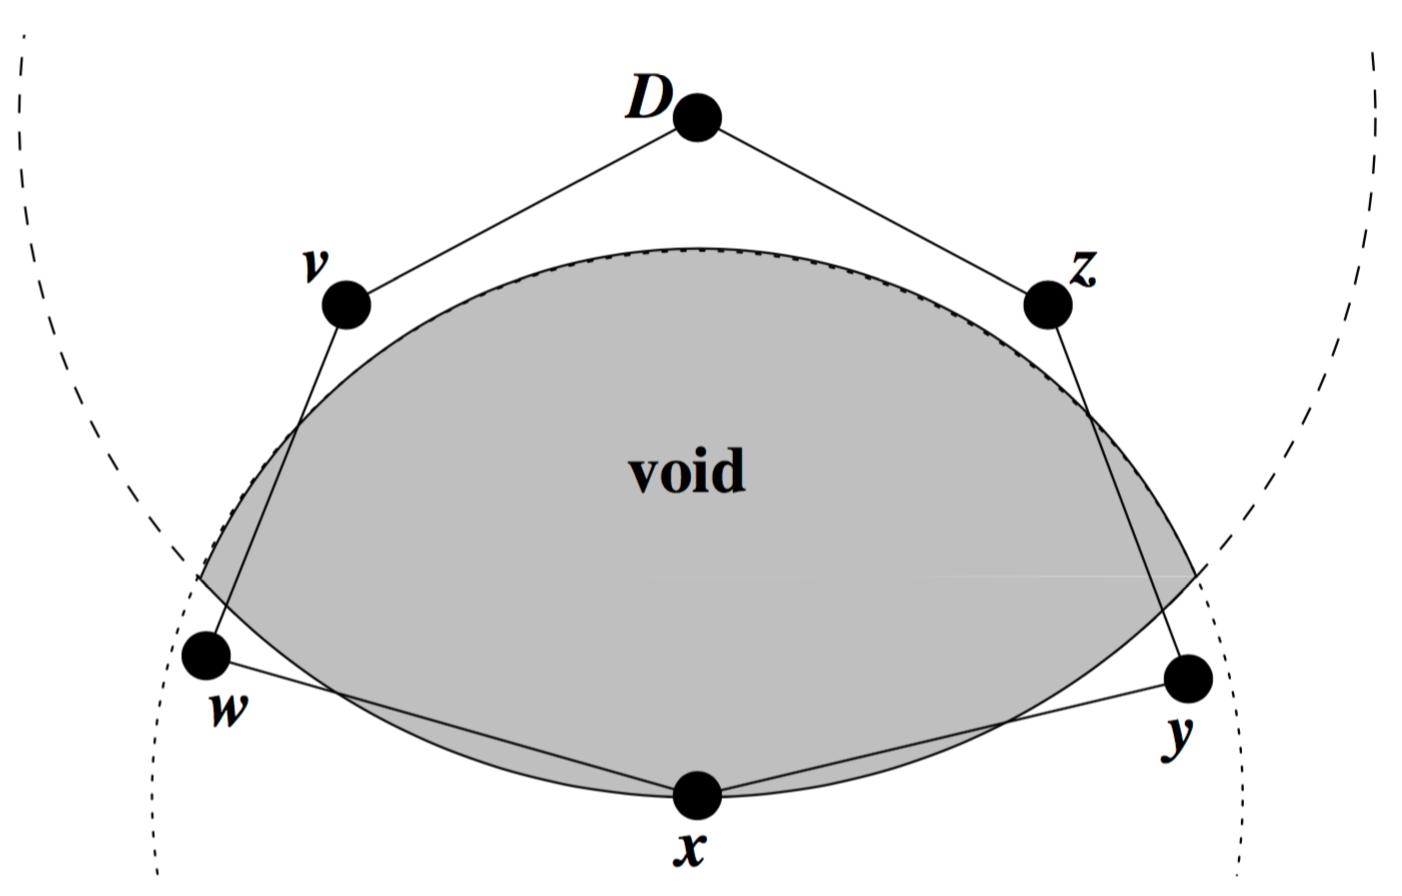
\includegraphics[width=0.4\textwidth]{Chapter1/Chapter1Figs/fig-local-minimum.png}
\caption{Node $x$’s void with respect to destination $D$.}
\label{local-minimum}
\end{figure}

A \emph{routing hole} in a wireless sensor network is a region where either there are no sensor nodes or the available nodes cannot participate in the activity of the network, i.e. they cannot communicate with the rest of the network. These holes can be formed either due to voids in sensor deployment or because of failure of sensor nodes due to various reasons such as malfunctioning, battery depletion or an external event such as fire, flood or structure collapse physically destroying the nodes. The local minimum phenomenon likely occurs when a routing hole is encountered. In the next chapter, we will discuss several previous works attempting to detect routing holes and to route the packet around them in greedy forwarding.
